\documentclass[10pt,letterpaper]{article}
\usepackage[top=1in,bottom=1in,left=1in,right=1in]{geometry}
\usepackage{datetime}
\usepackage{natbib}      % http://merkel.zoneo.net/Latex/natbib.php
\usepackage{palatino}
\usepackage{verbatim}
\usepackage[normalem]{ulem}
\bibpunct{(}{)}{;}{a}{,}{,}

\usepackage{array}

\usepackage{chngpage}
\usepackage{stmaryrd}
\usepackage{amssymb}
\usepackage{amsmath}
\usepackage{graphicx}
\usepackage{lscape}
\usepackage{subfigure}
\usepackage[usenames,dvipsnames]{color}
\definecolor{myblue}{rgb}{0,0.1,0.6}
\definecolor{mygreen}{rgb}{0,0.3,0.1}
\usepackage[colorlinks=true,linkcolor=black,citecolor=mygreen,urlcolor=myblue]{hyperref}

\newcommand{\bocomment}[1]{\textcolor{Bittersweet}{BO says: #1}}

\newcommand{\ignore}[1]{}
\newcommand{\transpose}{^\mathsf{T}}
\newcommand{\inner}[1]{\langle #1 \rangle} 
\newcommand{\smallsec}[1]{\noindent \textbf{#1\ }}
\newcommand{\cmd}[1] {{\color{blue}\texttt{#1}}}

\newcommand{\solution}[1]{{\color{myblue} \emph{[Solution:} 

#1 

\emph{End solution]}}}
\newcommand{\solutionnote}[1]{{\color{myblue} \emph{[Note:}

#1 

\emph{End note]}}}
\newcommand{\points}[1]{{\color{mygreen}\emph{[#1]\ \ }}}

\newcommand{\aone}{\diamondsuit}
\newcommand{\atwo}{\heartsuit}
\newcommand{\bone}{\triangle}
\newcommand{\btwo}{\Box}
\newcommand{\myand}{\ \land\ }
\newcommand{\myor}{\ \lor\ }
\newcommand{\mynot}{\lnot}

\title{
  Homework 2 \\
  \Large{CMPSCI 370 Spring 2019, UMass Amherst} \\
  \Large{Instructor: Subhransu Maji} \\
  \Large{TA: Tsung-Yu Lin}
}

\settimeformat{ampmtime}
\date{}
\begin{document}
\maketitle

\renewcommand\thesubsection{\thesection.\alph{subsection}}


\section*{Guidelines}

\paragraph{Submission.} Submit your answers via Gradescope that includes a pdf with your solutions and source code. You have a total of 3 late days for all your homework assignments which you can use in any way you like. However note that delay by even one minute counts as a full late day and submissions beyond the late days will not be given \emph{any} credit. Please contact the instructor and obtain permission ahead of time if you seek exceptions to the policy.

\paragraph{Plagiarism.} We might reuse problem set questions from previous years, covered by papers and webpages, we expect the students not to copy, refer to, or look at the solutions in preparing their answers. We expect students to want to learn and not google for answers. Any instance of cheating will lead to zero credit for the homework, and possibly a failure grade for the entire course.

\paragraph{Collaboration.} The homework must be done individually, except where otherwise noted in the assignments. 'Individually' means each student must hand in their own answers, and each student must write their own code in the programming part of the assignment. It is acceptable, however, for students to collaborate in figuring out answers and helping each other solve the problems. We will be assuming that you will be taking the responsibility to make sure you personally understand the solution to any work arising from such a collaboration.

\paragraph{Matlab requirements.} The code should work any Matlab version ($\geq$ 2011a) and relies on the Image Processing Toolbox for some functions.

\paragraph{Python requirements.} We will be using Python 2.7. The Python starter code requires \cmd{scipy}, \cmd{matplotlib} and \cmd{pillow} for loading images and \cmd{numpy} for matrix operations (at least v1.12). 
If you are not familiar with installing those libraries through some package manager (like \cmd{pip}), the easiest way of using them is installing \href{https://conda.io/docs/user-guide/install/index.html}{Anaconda}. Contact the course staff if you are having trouble installing these.

\paragraph{Using other programming languages.} We made the starter code in Python and Matlab. You are free to use other languages such as Octave or Julia with the caveat that these will not be supported by the course staff.




\newpage
\section{Light [30 points]}
\subsection{Linearity [5 points]}
Alice has a chandelier with 5 light
bulbs sockets. Currently, she has 5 100-watt incandescent bulbs in the sockets.
Each incandescent bulb is characterized by a spectrum $S_{\text{INC}}(\lambda)$, for integer $\lambda$
from 380 to 779, which gives the fraction of the total power output for each
interval with wavelengths between $\lambda$ and $\lambda + 1$ nanometers. For example, if
$S_{\text{INC}}(523) = 0.002$, then it means that the incandescent bulb outputs $0.002 \times
100 = .2$ watts in the range of $523$ -- $524$ nanometer wavelengths.
Eventually, she wants to replace the incandescent bulbs with fancy new
light emitting diode (LED) bulbs (also 100-watt bulbs) that have a different
spectrum $S_{\text{LED}}(\lambda)$, but right now, she only has 3 of these. She replaces 3 of the 5
incandescent bulbs with the LED bulbs. Give a formula for the chandelier’s new
spectrum $S_{\text{TOTAL}}$ in terms of the components of $S_{\text{INC}}$ and $S_{\text{LED}}$. The new spectrum
should give the fraction of the total power at each 1 nanometer portion of the
visible spectrum.


\subsection{Tristimulus theory [25 points]} Let $F_1$, $F_2$, and $F_3$ below
represent the power spectra of 3 different colored flashlights, where each of the 10 values is the fraction of power produced in a 40nm range from 380nm to 780nm. (Note: some of the power will be in the non-visible spectrum).\\

\begin{tabular}{c}
$F_1$ = [ 0.00, 0.01, 0.01, 0.02, 0.01, 0.02, 0.07, 0.29, 0.35, 0.12 ];\\
$F_2$ = [ 0.00, 0.01, 0.02, 0.11, 0.20, 0.25, 0.21, 0.10, 0.01, 0.00 ];\\
$F_3$ = [ 0.03, 0.10, 0.25, 0.27, 0.13, 0.02, 0.01, 0.01, 0.00, 0.00 ];\\
\end{tabular} \\

For example, flashlight F1 produces 12 percent of its power in the range 740-780nm. Figure~\ref{fig:spectra} shows the spectra of the three flashlights.\\

\begin{figure}[h]
\centering
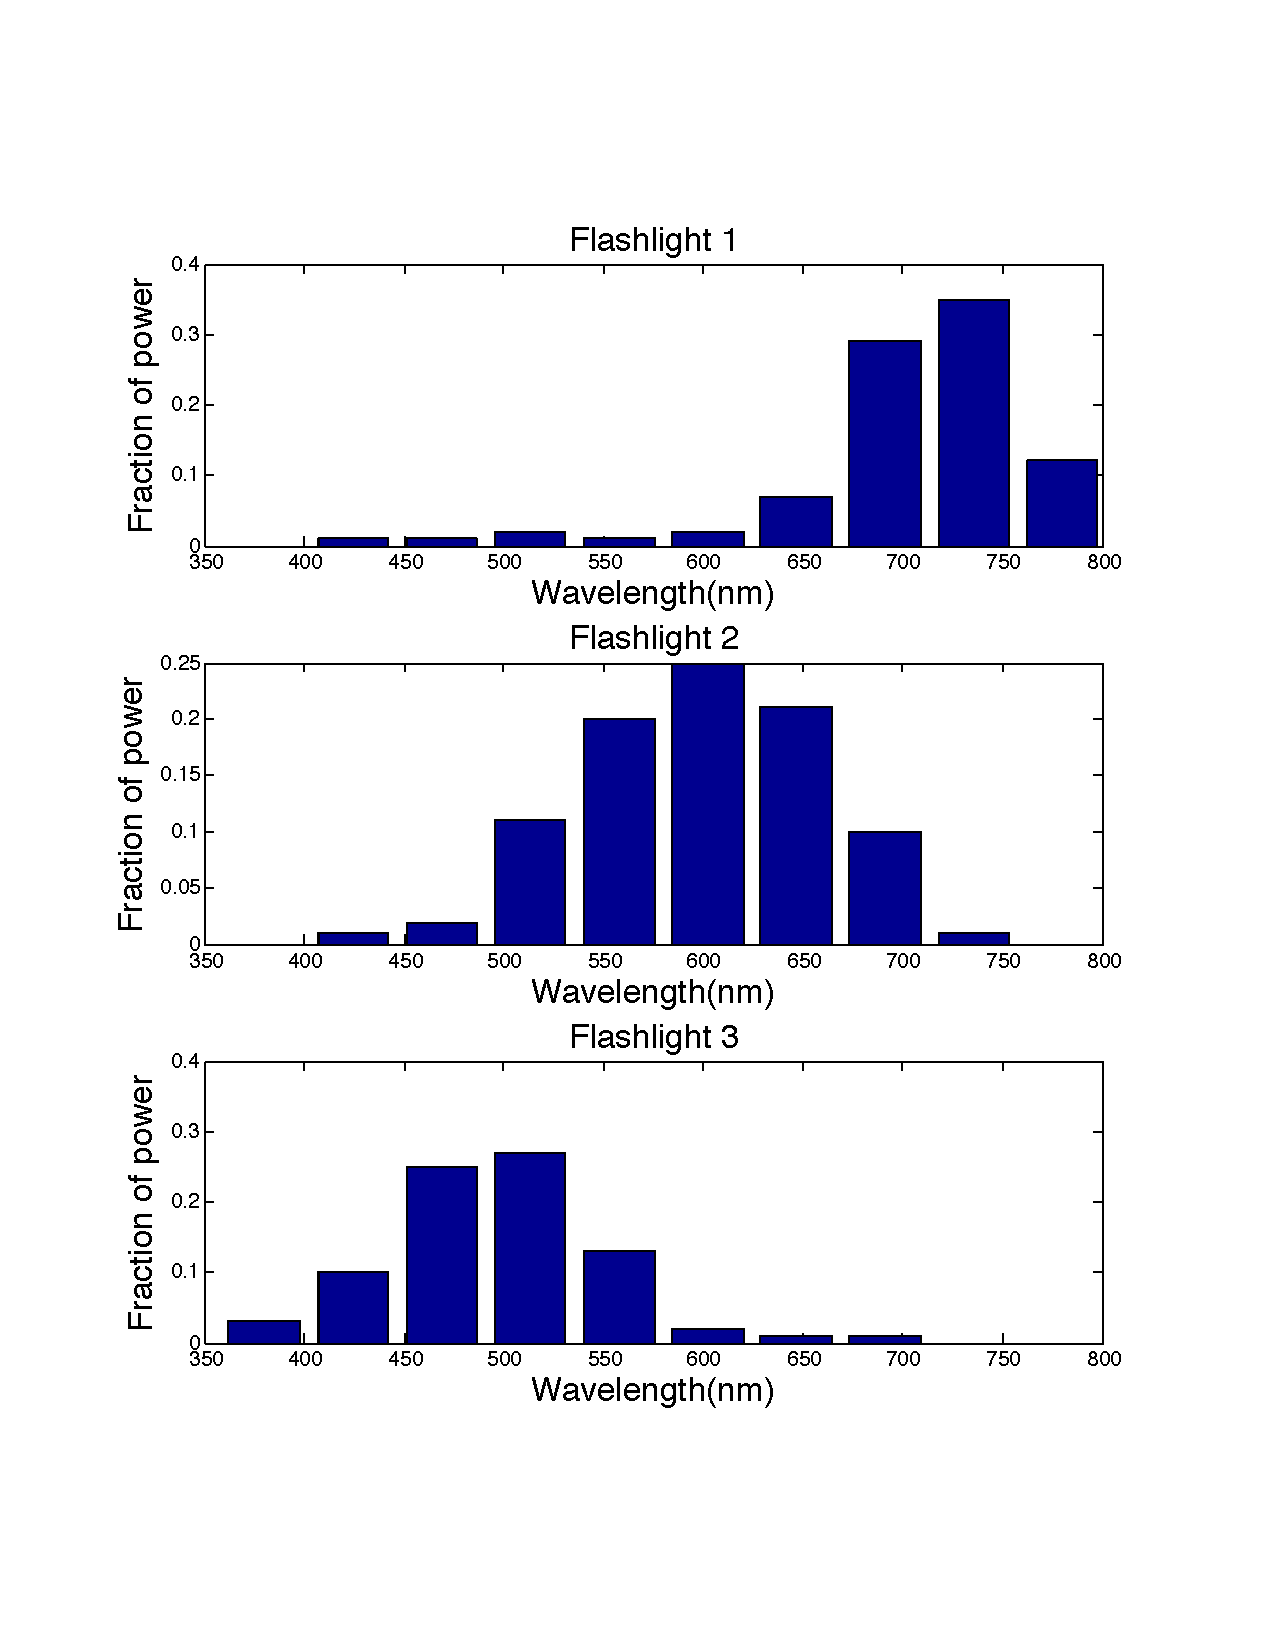
\includegraphics[width=0.5\linewidth]{flashlight-spectrum.pdf}
\caption{\label{fig:spectra}\textbf{Three flashlight spectra.} This image shows the three spectra of $F_1$, $F_2$, and $F_3$.}
\end{figure}

Let $S_r(\lambda)$, $S_g(\lambda)$, and $S_b(\lambda)$ represent the relative absorption spectra of the cone cells in your eye. This means that, of the power absorbed by a given type of cone cell, the fraction absorbed in a given range is given by these numbers.\\

\begin{tabular}{c}
$S_r(\lambda)$ = [ 0.16, 0.26, 0.28, 0.15, 0.10, 0.03, 0.02, 0.00, 0.00, 0.00 ]; \\
$S_g(\lambda)$ = [ 0.00, 0.00, 0.04, 0.23, 0.34, 0.23, 0.15, 0.01, 0.00, 0.00 ];\\
$S_b(\lambda)$ = [ 0.00, 0.00, 0.00, 0.00, 0.01, 0.04, 0.08, 0.23, 0.35, 0.29 ];
\end{tabular}\\

When a flashlight is 5 meters from a white screen, assume that it stimulates
a cone cell response (relative to the maximum possible response from that cone)
given by: \\
\begin{equation*}
R^f_c = \sum_{i=1}^{10} F_f (i) \times S_c(i).
\end{equation*}

Here $F_f$ is flashlight $f$, $S_c$ is the absorption spectrum for cones of type $c$, and $R^f_c$ is the response for cone cell type $c$ and flashlight $f$. For example, from 5 meters away, the third flashlight $F_3$ generate a response from the green cone cells of\\
\begin{eqnarray*}
R^3_g &=& \sum_{i=1}^{10} F_3 (i) \times S_g(i) \\
&=& 0.03\times0.00 + 0.10\times0.00 + 0.25\times0.04 + 0.27\times0.23 + 0.13\times0.34 + \\ 
&~& 0.02\times0.23 + 0.01\times0.15 + 0.01\times0.01 + 0.00\times0.00 + 0.00\times0.00 \\
&=& 0.1225\\
\end{eqnarray*}

Consider the response of all 3 cone cell types at once to a given flashlight $f$
at a fixed distance from the white screen. We will call this variable $R^f$, and it will be a vector of 3 values:
\[
	R^f = \left[ \begin{array}{c}
				R^f_r \\
				R^f_g \\				
				R^f_b \end{array} \right]
\]

Of course, the “color” that you see for a particular flashlight will be related
to the cone cell responses $R^f$ produced by that flashlight. Due to the linearity
of light and the approximate linearity of cone cell responses, you can model the
responses of the cone cells to two flashlights, say 1 and 3, as

\[
	R^1 + R^3 = \left[ \begin{array}{c}
				R^1_r + R^3_r\\
				R^1_g + R^3_g\\				
				R^1_b + R^3_b\end{array} \right]
\]

\begin{enumerate}
\item \textbf{(10 points)} Let the matrix R be defined to be 
\[
	R = \left[ \begin{array}{ccc}
				R^1_r &  R^2_r & R^3_r\\
				R^1_g &  R^2_g & R^3_g\\
				R^1_b &  R^2_b & R^3_b\end{array} \right]
\]
Write a Matlab or Python function to compute the matrix $R$ given $F_1$, $F_2$, $F_3$, $S_r$, $S_g$, and $S_b$. Give the value of the matrix $R$.


\item \textbf{(15 points)} If we had a way to make each flashlight brighter or dimmer, then we could
create novel color combinations. In particular, if we let $b_1$ be the brightness
multiplier for flashlight 1, $b_2$ the brightness multiplier for flashlight 2, and $b_3$ the brightness multiplier for flashlight 3, then we can create arbitrary linear
combinations of the 3 flashlights as
\[
	b_1R^1 + b_R^2 + b_3R^3 = \left[ \begin{array}{c}
				b_1R^1_r + b_2R^2_r + b_3R^3_r\\
				b_1R^1_g + b_2R^2_g + b_3R^3_g\\				
				b_1R^1_b + b_2R^2_b + b_3R^3_b\end{array} \right]
\]

Now suppose you want to create a combination of lights that results in a
particular perceived color. For example, the color turquoise is perceived when
the RGB cone cells have a response of
\[
C_{\text{turquoise}} = \left[ \begin{array}{c} 0.2896 \\ 0.8862 \\ 0.7471 \end{array} \right]
\]

We need to solve the following set of equations
\begin{eqnarray*}
b_1R^1_r + b_2R^2_r + b_3R^3_r = C_r\\
b_1R^1_g + b_2R^2_g + b_3R^3_g = C_g \\
b_1R^1_b + b_2R^2_b + b_3R^3_b = C_b \\
\end{eqnarray*}
This can be written in matrix form as
\[ Rb = C, \]

where $R$ is the matrix defined previously, $b$ is a vector of 3 multiplier values, and $C$ is the 3 color components for the desired color. Fortunately, this is extremely easy to solve in Matlab! By multiplying both sides by the matrix inverse of $R$, we obtain
\[ R^{-1}Rb = R^{-1}C, \]
and then simplifying,
\[ b = R^{-1}C. \]
In Matlab, the inverse of a matrix can be obtained by simply raising the matrix to the power -1.
In Python, you can use the function \cmd{np.linalg.inv()}.

Write a Matlab or Python function, which, given the matrix $R$ and a
set of desired color responses in the form of a vector $C$ calculates the proper
brightness multiplier weights $b$ and returns them as a single vector of 3 values. Using this code compute the multiplier weights for each flashlight so that you  obtain:

Turquoise: 
\[
C_{\text{turquoise}} = \left[ \begin{array}{c} 0.2896 \\ 0.8862 \\ 0.7471 \end{array} \right]
\]\\

$b_1$: \underline{\hspace{3cm}}, $b_2$: \underline{\hspace{3cm}}, $b_3$:\underline{\hspace{3cm}}

\vspace{0.5in}
Goldenrod (a slightly brownish yellow): 
\[
C_{\text{goldenrod}} = \left[ \begin{array}{c} 0.8567 \\ 0.6874 \\ 0.1408 \end{array} \right]
\]\\

$b_1$: \underline{\hspace{3cm}}, $b_2$: \underline{\hspace{3cm}}, $b_3$:\underline{\hspace{3cm}}

\end{enumerate}


\section{White balance [20 points]}
White balance is the process of removing unrealistic color casts which appear because the light when the picture was taken (e.g. sunlight) does not match the color of the light you are viewing the picture in (e.g. LED bulb). Our eyes are very good at removing the effect of illumination to judge the true color of an object (a.k.a. color constancy). A simple way of modeling the effect of a light on a surface is to assume that the reflected color $I = (i_r,i_g,i_b)$ arises due to light of color $L= (l_r,l_g,l_b)$ interacting with paint of color $C = (c_r,c_g,c_b)$ satisfying  
	$L \times C = I$, i.e. 
	\[ (l_r \times c_r,l_g \times c_g ,\l_b \times c_b) = (i_r,i_g,i_b)
	\]
Assume $l_r, l_g, l_b \in [0, 1]$ is the fractional power of the light in each of the color channels. Given the light value $L$ at a given pixel we can obtain its true color by dividing the measured intensity with the light 
\[
	c_r = \frac{i_r}{l_r}; 
	c_g = \frac{i_g}{l_g}; 
	c_b = \frac{i_b}{l_b}; 
\]

In general, computing $L$ and $C$ given $I$ is ill-posed. For example, a red pixel of value $I=(255,0,0)$ could be due to a white light $L=(1,1,1)$ illuminating a red object $C=(255,0,0)$, or red light $L=(1,0,0)$ illuminating a white object $C=(255,255,255)$. Both these satisfy $L\times C = I$.

We need priors to this ambiguity. One such prior is the "gray world" assumption that states the average pixel color under white light is gray. Recall that any color $(r,g,b)$ where $r=g=b$ is gray. For the purposes of this homework we will assume that the average is $(128,128,128)$ (assuming that the values are between 0 and 255) and that the light is uniform across all pixels.

\begin{itemize}
\item \textbf{(5 points)} Show that under the gray world assumption the color of the light $L$ is given by 
\[
	L = \left(\frac{r_{ave}}{128}, \frac{g_{ave}}{128}, \frac{b_{ave}}{128}\right),
\]

where, $r_{ave}, g_{ave}, b_{ave}$ are the average of the red, green, and blue channels of the image, and thus  you can obtain the true color of a pixel as
\[
	c_r = i_r \times \frac{128}{r_{ave}}; 
	c_g = i_g \times \frac{128}{g_{ave}}; 
	c_b = i_b \times \frac{128}{b_{ave}}; 
\]

\item \textbf{(15 points)} Implement a function $\cmd{[L, C] = grayworld(I)}$ that takes an image $\cmd{I}$ and returns the light $L$ and color image $C$ using the above calculations. Run your code on the image $\cmd{wb\_sardmen-incorrect.jpg}$ included in the \cmd{data} directory, as seen in Figure~\ref{fig:color}.  
Write down the value of $L$ in the format shown below in your solutions, include the code for the function and a picture of the color corrected image $C$. 
Note that the color corrected image will need to be scaled back to the range of [0,255] or [0,1] to display properly using \cmd{imshow()} in Matlab. A simple way of doing this is to divide all the values by the maximum pixel value across all channels and scale it back to the appropriate range.
Alternatively you can use the \cmd{imagesc(C);} command in Matlab that scales the or \cmd{plt.imshow(C); plt.show()} in Python with the appropriate arguments that will automatically scale the ranges.

Notice that if your image is loaded in a floating point format with intensities between 0 and 1, a white pixel has value $(1.0, 1.0, 1.0)$ and the average can be assumed to be $(0.5, 0.5, 0.5)$.\\ 
\textbf{Light}~~ $l_r$: \underline{\hspace{2cm}}, $l_g$: \underline{\hspace{3cm}}, $l_b$:\underline{\hspace{3cm}}
\end{itemize}

\begin{figure}[h]
\centering
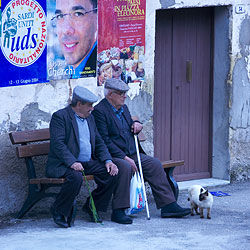
\includegraphics[scale=1]{../data/wb_sardmen-incorrect.jpg}
\caption{\label{fig:color} Image with a color cast. Source \url{ http://www.cambridgeincolour.com/tutorials/white-balance.htm}}
\end{figure}

\section{Hybrid images [20 points]}
A hybrid image is a superposition of a low-pass filtered (i.e. blurry) version of the one image and a high-pass filtered (i.e. sharp) version of a second image that looks like one or the other depending on the perceived resolution of the image. In this part you will try to create such images.


Recall that one can obtain a sharp image by subtracting the blurry version of an image from itself. Mathematically we have
\[
	I = \texttt{blurry}(I) + \texttt{sharp}(I).
\]

The low-pass filtered image can be obtained by filtering an image with a Gaussian. In Matlab the function $\cmd{fspecial('gaussian', hsize, sigma)}$ returns a Gaussian filter of standard deviation $\cmd{sigma}$ approximated as a filter of size 
$\cmd{[hsize hsize]}$.
In Python, we added a function \cmd{gaussian(hsize, sigma)} to \cmd{utils.py} that performs exactly the same way. 
A good rule of thumb is to set the filter size as $\cmd{hsize = 6*sigma+1}$. 
You can also obtain the filter using the formula of the Gaussian function.
The $\cmd{imfilter}$ function in Matlab implements the image filtering/convolution function. 
In Python, the function \cmd{convolve} from \cmd{scipy.ndimage.filters} does the same. 
The filtering of a color image can be obtained by filtering each channel separately or replicating the Gaussian filter across channels.


Thus a hybrid image of $I_1$ and $I_2$ can be obtained by
\begin{equation}\label{eq:hybrid}
	I_{hybrid} = blurry(I_1, \sigma_1) + sharp(I_2, \sigma_2) = I_1 * g(\sigma_1) + I_2 - I_2*g(\sigma_2)
\end{equation}

where, $g(\sigma_1)$ and $g(\sigma_2)$ are Gaussian filters with parameters $\sigma_1$ and $\sigma_2$ and * denotes the filtering operator. Figure~\ref{fig:blur} shows the result of convolution with Gaussian filters with two different values of $\sigma$. 
The filters were obtained in Matlab by typing $\cmd{f = fspecial('gaussian', 6*s + 1, s)}$ and \cmd{f = gaussian(6*s + 1, s)} in Python (remember to import the function from \cmd{utils}).


\begin{figure}
\begin{tabular}{cccc}
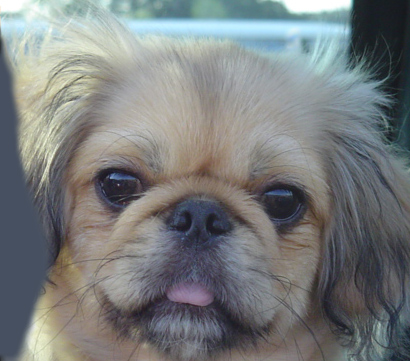
\includegraphics[width=0.23\linewidth]{../output/dog.jpg} &
\includegraphics[width=0.23\linewidth]{../output/dog-blurry-4.jpg} & 
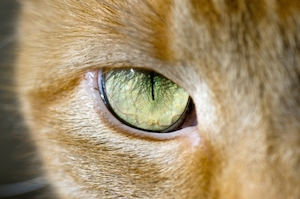
\includegraphics[width=0.23\linewidth]{../output/cat.jpg} &
\includegraphics[width=0.23\linewidth]{../output/cat-blurry-10.jpg}\\
dog image & $\sigma=4$ & cat image & $\sigma=10$ \\
\end{tabular}
\caption{\label{fig:blur} Effect of filtering with a Gaussian. The bigger the sigma the more blurry it is.}
\end{figure}

\begin{itemize}

\item \textbf{(20 points)} Implement the function 
$\cmd{hybridImage(im1, im2, sigma1, sigma2)}$ that computes the hybrid image using Equation~\ref{eq:hybrid}. Use your code to generate at least one example of a hybrid image (see examples here \url{http://cvcl.mit.edu/hybrid_gallery/gallery.html}). You will have to tune the $\cmd{sigma1}$ and $\cmd{sigma2}$ to make it work on specific images. In order to visualize the hybrid image it is sometimes useful to show multiple copies of the image at different resolutions. The codebase includes a helper function $\cmd{vis\_hybrid\_image}$ which can be used to create such a figure.
In Python, \cmd{matplotlib} does not handle negative values in images like Matlab does, so remember to use \cmd{np.clip} to make sure that image values are between 0 and 1.
Include the code, the two source images, the hybrid image displayed in the format below, as well as the parameters that worked for you. The top three submissions (judged based on creativity and compellingness of the hybrid image) will be announced in class.

\end{itemize}
\begin{figure}[h]
\includegraphics[width=\linewidth]{../output/hybrid-4-10.jpg}
\caption{Hybid image of the dog and cat. The large image looks like the cat while the small image looks like the dog. The image was created with $\sigma_1 = 4$ and $\sigma_2 = 10$.}
\end{figure}
\end{document}
